\documentclass[a4paper,14pt]{extarticle} \usepackage[utf8]{inputenc}
\usepackage[T1]{fontenc}
\usepackage[margin=2.5cm]{geometry}

% Fonte Caladea se existir, senão lmodern
\IfFileExists{caladea.sty}{
  \usepackage{caladea}
}{
  \usepackage{lmodern} }
\usepackage{ragged2e}
\usepackage{graphicx}
\usepackage[portuguese]{babel}
\usepackage{wrapfig}
\usepackage{hyperref}
\usepackage{fancyhdr}
\usepackage{xcolor}
\usepackage{rotating}
\usepackage{titlesec}
\usepackage{epigraph}
\usepackage{dirtytalk}
\usepackage{indentfirst} % Indenta o primeiro parágrafo após seções

% Ajuste do recuo de parágrafo
\setlength{\parindent}{1.5em}

% Centralizar títulos
\titleformat{\section}
  {\normalfont\centering\bfseries\Large}{}{1em}{}

\titleformat{\subsection}
  {\normalfont\centering\bfseries\large}{}{1em}{}

\titleformat{\subsubsection}
  {\normalfont\centering\bfseries}{}{1em}{}

% -------------- Símbolos de Versículo e Resposta --------------
% Definição do símbolo (a “barrinha” inclinada)
\makeatletter
\newcommand{\vers@resp@sym}{%
  \raisebox{0.2ex}{\rotatebox[origin=c]{-20}{$\m@th\rceil$}}%
}
% macro interna que sobrepõe a barrinha e a letra V ou R
\newcommand{\vers@resp}[2]{%
  {\ooalign{%
     \hidewidth\kern#1\vers@resp@sym\hidewidth\cr
     #2\cr
  }}%
}
% comandos públicos \versicle e \response
\DeclareRobustCommand{\versicle}{\vers@resp{-0.1em}{V}}
\DeclareRobustCommand{\response}{\vers@resp{0pt}{R}}
\makeatother
% ^------------- Símbolos de Versículo e Resposta -------------^

% Rodapé com imagem e página
\pagestyle{fancy}
% ---- Cabeçalho ------------
\fancyhf[C]{}
% ----- Rodapé --------------
\fancyfoot[LO,LE]{%
  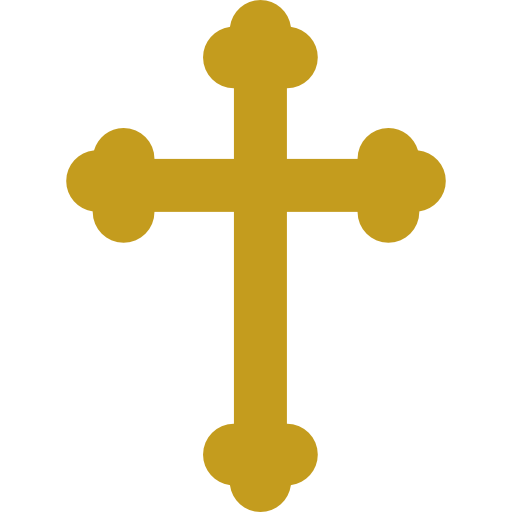
\includegraphics[scale=0.2]{assets/cross.png}\quad
  \textit{\textit{São Cirilo e São Metódio, Rogai por Nós}}
}
\fancyfoot[RO,RE]{\thepage}

\usepackage{pdfpages}
\begin{document}
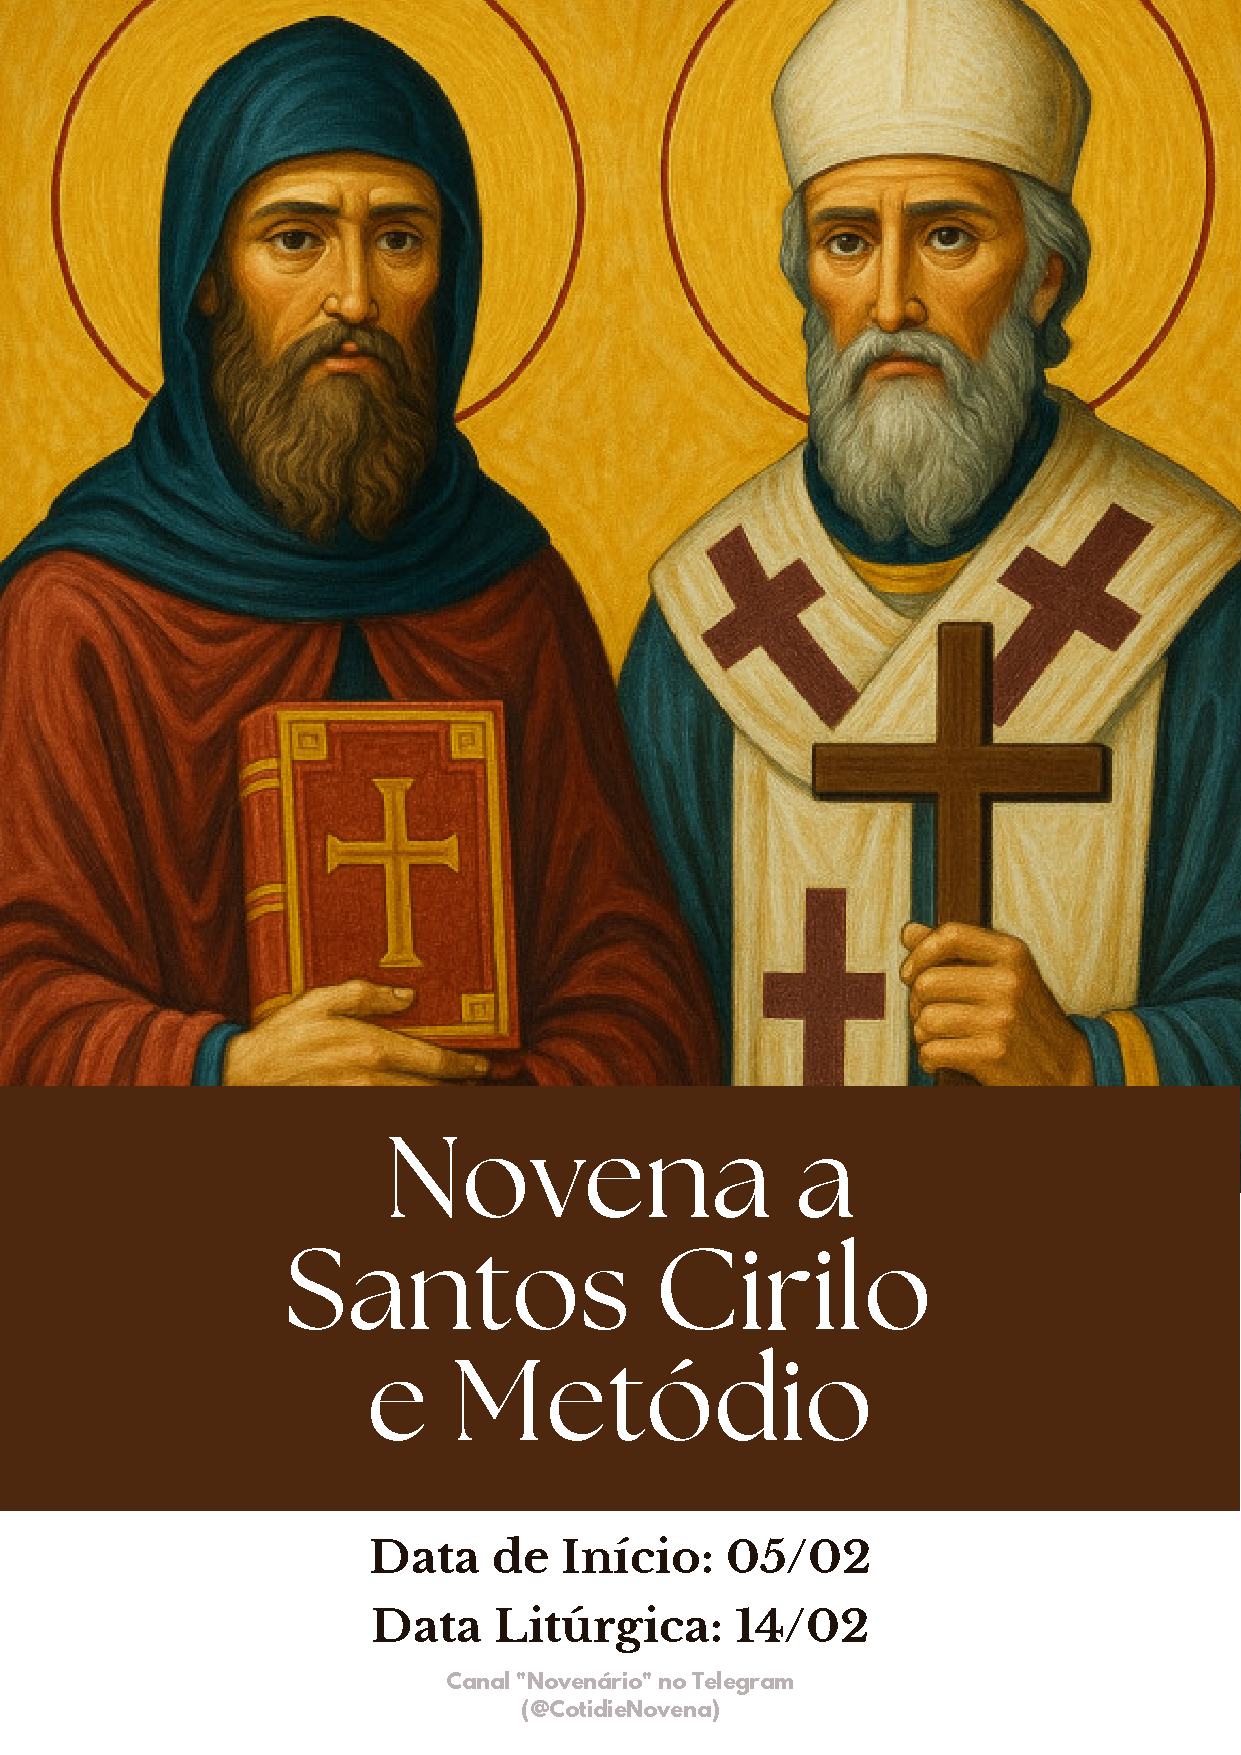
\includepdf[pages=1]{Capa Santos Cirilo e Metódio}


\begin{center}
  {\huge Novena dos Santos Cirilo e Metódio}
\end{center}



\noindent\rule{\textwidth}{0.4pt}
\tableofcontents
\thispagestyle{empty}


% --- Origem ---
\newpage

\section{História}
Uma vida constantemente em viagem, muito cansativa, entre as aventuras e os perigos de dois homens unidos pelo vínculo de sangue, da fé cristã, do destino de dever traçar um caminho novo onde a tradição já havia pavimentado uma estrada larga e movimentada. Tem disto e muito mais por trás da auréola e a pose hierática com os quais são retratados talvez os mais célebres irmãos Santos da catolicidade, Cirilo e Metódio.
\subsection{O administrador e o erudito}

Apenas dois anos separam os nascimentos. O maior é Metódio (que na realidade se chamava Miguel) e nasce em 825 em Tessalonica, onde em 827 vem à luz Cirilo (no século, Constantino). A história os vê inicialmente divididos. O primeiro se distingue logo como um hábil administrador e recebe o cargo de arconte de uma província do Império bizantino.

O segundo recebe uma educação refinada em Constantinopla - gramática, retórica, astronomia e música – o que deveria fazer dele um alto dignatário imperial. Mas quando chega o tempo, Cirilo tem uma ideia diferente e recusa.

\subsection{O novo alfabeto da Bíblia}

Por volta dos 35 anos, o Imperador Miguel III pensa em Cirilo quando os Czares do Mar de Azov pedem o envio de um letrado que saiba discutir com Judeus e sarracenos. É aqui que os dois irmãos se reúnem, iniciando a primeira de inúmeras missões juntos.

Dois anos mais tarde, em 863, é a vez da Grande Morávia. O objetivo da missão é a de opor-se à influência germânica com dois missionários que soubessem o eslavo.

Mas Cirilo e Metódio vão além. Provavelmente percebendo as dificuldades de comunicar as Escrituras nas línguas oficiais, o latim e o grego, os dois irmãos criam um novo alfabeto, o “glagolítico”, universalmente conhecido como “cirílico”: 40 caracteres derivados na maior parte de grafemas de cursiva medieval do alfabeto grego.

\subsection{Evangelho do leste}

A obra deles é tão extraordinária que o Papa, chamando-os a Roma, recebe Cirilo e Metódio indo ao encontro deles em procissão.

Os grandes esforços aos quais se submeteram, debilitam a saúde do mais jovem. Em 14 de fevereiro de 869 Cirilo, que tornou-se monge, morre após uma doença.

Metódio é consagrado bispo e continua a missão de sempre, superando hostilidades e incompreensões, e instruindo discípulos na tradução dos textos sagrados.

% --- Orações Diárias ---
\newpage


\vfill

\section{Orações}
\subsection{Oração Inicial}\label{sub:inicial} % (fold)

Ó São Cirilo e São Metódio, apóstolos dos eslavos e grandes missionários, vocês dedicaram suas vidas à evangelização e à promoção da fé cristã entre os povos que não conheciam o Evangelho. Com coragem e determinação, vocês criaram um novo alfabeto eslavo e traduziram as Escrituras, tornando possível que muitos pudessem ouvir a Palavra de Deus em sua própria língua. Ao longo desta novena, pedimos que intercedam por nós, ajudando-nos a viver com o mesmo fervor missionário e amor ao próximo que vocês demonstraram. Que possamos ser instrumentos da paz e da esperança em nosso mundo. Amém.


\subsubsection{Dia 1}
\underline{\nameref{sub:inicial}}

\textbf{A Chamada à Missão}

Ó São Cirilo, você foi chamado para ser um mensageiro do Evangelho desde jovem. Sua disposição em deixar tudo para seguir a missão é um exemplo para todos nós. Que sua intercessão nos ajude a ouvir o chamado de Deus em nossas vidas e a responder com prontidão.

\underline{\nameref{sub:final}}

\subsubsection{Dia 2}
\underline{\nameref{sub:inicial}}

\textbf{A Importância da Educação}

São Metódio, você dedicou sua vida à educação dos povos eslavos. Sua sabedoria e conhecimento foram fundamentais para a formação espiritual das comunidades que evangelizou. Que sua intercessão nos inspire a valorizar o aprendizado e a partilhar o conhecimento com generosidade.

\underline{\nameref{sub:final}}

\subsubsection{Dia 3}
\underline{\nameref{sub:inicial}}

\textbf{A Criação do Alfabeto}

Ó São Cirilo, sua criação do alfabeto cirílico foi um ato de amor pela cultura eslava. Você reconheceu a importância de comunicar as verdades de Deus na língua do povo. Que sua intercessão nos ajude a valorizar nossa própria cultura enquanto proclamamos o Evangelho.

\underline{\nameref{sub:final}}

\subsubsection{Dia 4}
\underline{\nameref{sub:inicial}}

\textbf{Coragem nas Adversidades}

São Metódio, você enfrentou hostilidades e incompreensões durante sua missão. Sua coragem em permanecer firme na fé é um exemplo poderoso para todos nós. Que sua intercessão nos dê força para enfrentar os desafios que surgem em nossa caminhada cristã.

\underline{\nameref{sub:final}}

\subsubsection{Dia 5}
\underline{\nameref{sub:inicial}}

\textbf{A Luz da Esperança}

Ó gloriosos irmãos, vocês trouxeram esperança aos que estavam perdidos. Sua mensagem de amor e salvação é uma luz que brilha no mundo. Que possamos ser portadores dessa esperança onde quer que estejamos.

\underline{\nameref{sub:final}}

\subsubsection{Dia 6}
\underline{\nameref{sub:inicial}}

\textbf{A Perseverança na Oração}

São Cirilo e São Metódio, vocês sabiam que a oração era fundamental para fortalecer a missão. Que sua intercessão nos ajude a ser perseverantes na oração e a buscar sempre uma relação mais profunda com o Senhor.

\underline{\nameref{sub:final}}

\subsubsection{Dia 7}
\underline{\nameref{sub:inicial}}

\textbf{O Amor ao Próximo}

Ó irmãos santos, vocês viveram o mandamento do amor ao próximo. Sua compaixão pelos necessitados é um testemunho vivo da caridade cristã. Que sua intercessão nos inspire a agir com generosidade e cuidar dos mais pobres entre nós.

\underline{\nameref{sub:final}}

\subsubsection{Dia 8}
\underline{\nameref{sub:inicial}}

\textbf{A Unidade na Igreja}

São Metódio, você trabalhou incansavelmente pela unidade da Igreja. Sua determinação em promover a paz entre os povos é um exemplo para todos nós. Que sua intercessão nos ajude a promover a unidade entre os cristãos e a superar divisões que nos afastam uns dos outros.


\underline{\nameref{sub:final}}

\subsubsection{Dia 9}
\underline{\nameref{sub:inicial}}

\textbf{A Celebração da Vida Nova}

Ó São Cirilo e São Metódio, celebramos hoje as graças recebidas através de suas vidas. Sua dedicação ao Evangelho nos lembra da importância de viver plenamente nossa fé. Que possamos sempre renovar nosso compromisso com Cristo e viver como verdadeiros discípulos.


\underline{\nameref{sub:final}}

\subsection{Oração Final}\label{sub:final} % (fold) \subsection{Orações de Cada Dia}

Ó São Cirilo e São Metódio, agradecemos por seu exemplo de amor incondicional e coragem na defesa da fé. Pedimos que intercedam por nós junto ao Senhor Jesus para que possamos viver com determinação na nossa caminhada cristã. Ajude-nos a amar uns aos outros como Cristo nos amou e a sermos luz no mundo através das nossas ações. Que pela sua intercessão possamos receber as graças necessárias para crescer na fé e no amor divino todos os dias de nossas vidas. Amém.

\[\textbf{Pai-Nosso, Ave-Maria, Glória}\]


\vfill

\begin{center}
\subsection*{Fontes:}
Adaptado de: {\color{blue} \underline{\href{https://www.vaticannews.va/pt/santo-do-dia/02/14/ss--cirilo--monge-e-metodio--bispo---padroeiros-da-europa-.html}{Vatican News}}} e {\color{blue} \underline{\href{https://www.youtube.com/playlist?list=PLN7jQwkJvdQrb9mji8dOObIvV0iK1W7uU}{A Oração dos Santos}}}
\end{center}


\end{document}
